\documentclass[tikz,border=10pt]{standalone}
\usepackage{tkz-euclide} % 用于辅助几何点位计算

\begin{document}
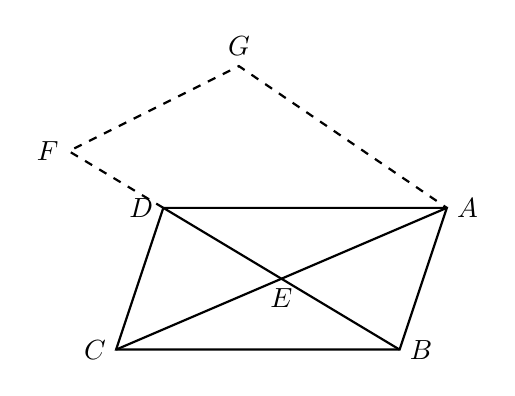
\begin{tikzpicture}[scale=1.2, >=stealth, thick]

    % 1. 定义核心顶点坐标 (平行四边形 ABCD)
    \coordinate (C) at (0, 0);
    \coordinate (B) at (3, 0);
    \coordinate (A) at (3.5, 1.5);
    \coordinate (D) at (0.5, 1.5); % 满足 AB // CD 且 AD // BC

    % 2. 计算对角线交点 E
    \coordinate (E) at (intersection of A--C and B--D);

    % 3. 定义虚线平行四边形 AEFG 的顶点
    % 根据原图，G 在 A 的左上方，F 在 D 的左上方
    \coordinate (G) at (1.3, 3);
    \coordinate (F) at (-0.5, 2.1); 
    % 确保 G-A 向量与 F-E 向量一致，且 EF // AG

    % 4. 绘制实线部分 (平行四边形 ABCD 及其对角线)
    \draw (A) -- (B) -- (C) -- (D) -- cycle;
    \draw (A) -- (C);
    \draw (B) -- (D);

    % 5. 绘制虚线部分 (平行四边形 ADFG)
    \draw[dashed] (D) -- (F) -- (G) -- (A);

    % 6. 标注顶点标签
    % 使用 pos 和 anchor 精细调整标签位置，避免遮挡线条
    \node[right] at (A) {$A$};
    \node[right] at (B) {$B$};
    \node[left]  at (C) {$C$};
    \node[left]  at (D) {$D$};
    \node[below] at (E) {$E$};
    \node[left]  at (F) {$F$};
    \node[above] at (G) {$G$};

\end{tikzpicture}
\end{document}